\chapter[Introduction]{Introduction}
%\addcontentsline{toc}{chapter}{Chapter 1\\Introduction}
\label{chapter:introduction}
\pagenumbering{arabic}

In chapter \ref{chapter:introduction},  present spectrum scarcity problem as the background of this thesis and technology proposed for solution is described. Aslo, the overview of this thesis and purpose is described. 
\section{Background}
 Due to the rapid development of wireless communication systems, a demand on sprectrum resource for communication has increased explosively. Because the data rate and perfomance of the wireless communication system, such as mobile phone, are improved, it leads to a serious sprectrum scarcity problem.

 From Fig. \ref{fig:Cisco}, reference \cite{ref:Cisco} predicts that Global mobile data traffic will increase nearly tenfold between 2014 and 2019 and mobile data traffic will grow at a compound annual growth rate (CAGR) of 57 percent from 2014 to 2019, reaching 24.3 exabytes per month by 2019. 
\begin{figure}[!htp]
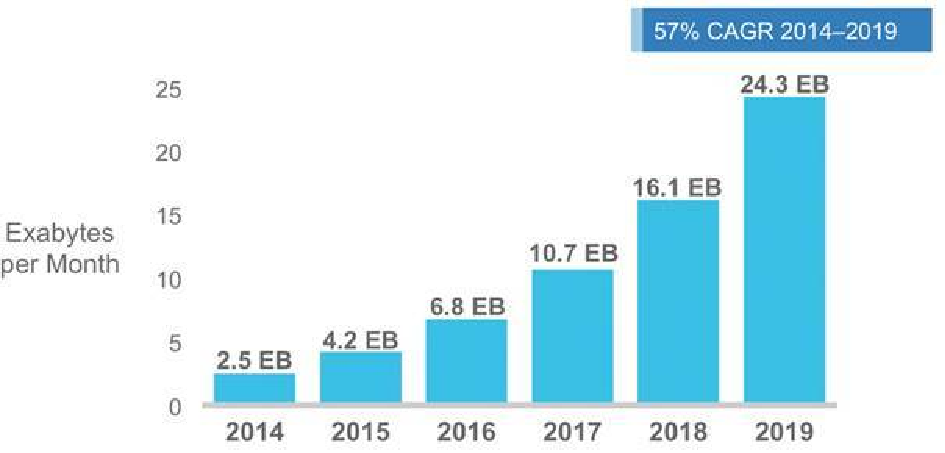
\includegraphics[width=150mm,clip]{traffic_trend.pdf}
\caption{Cisco Forecasts 24.3 Exabytes per Month of Mobile Data Traffic by 2019}
\label{fig:Cisco}
\end{figure}
In addition to the increasement of the data traffic, a fixed resource allocation method as the current spectrum allocation policy, which is utilized for avoiding harmful interference toward licensed systems with each other, is also considered as a major reason for the scarcity of the spectrum resource. As a reason, almost linear increasing demand on necessary bandwidth for communication leads to a difficult allocation for new systems. From Fig. \ref{fig:MIC} reported from Ministry of Internal Affairs and Communications(MIC) in Japan government, it is shown that most of the spectrum resources has already been allocated. Thus, the lack of spectrum resources has become a serious problem.
\begin{figure}[!htp]
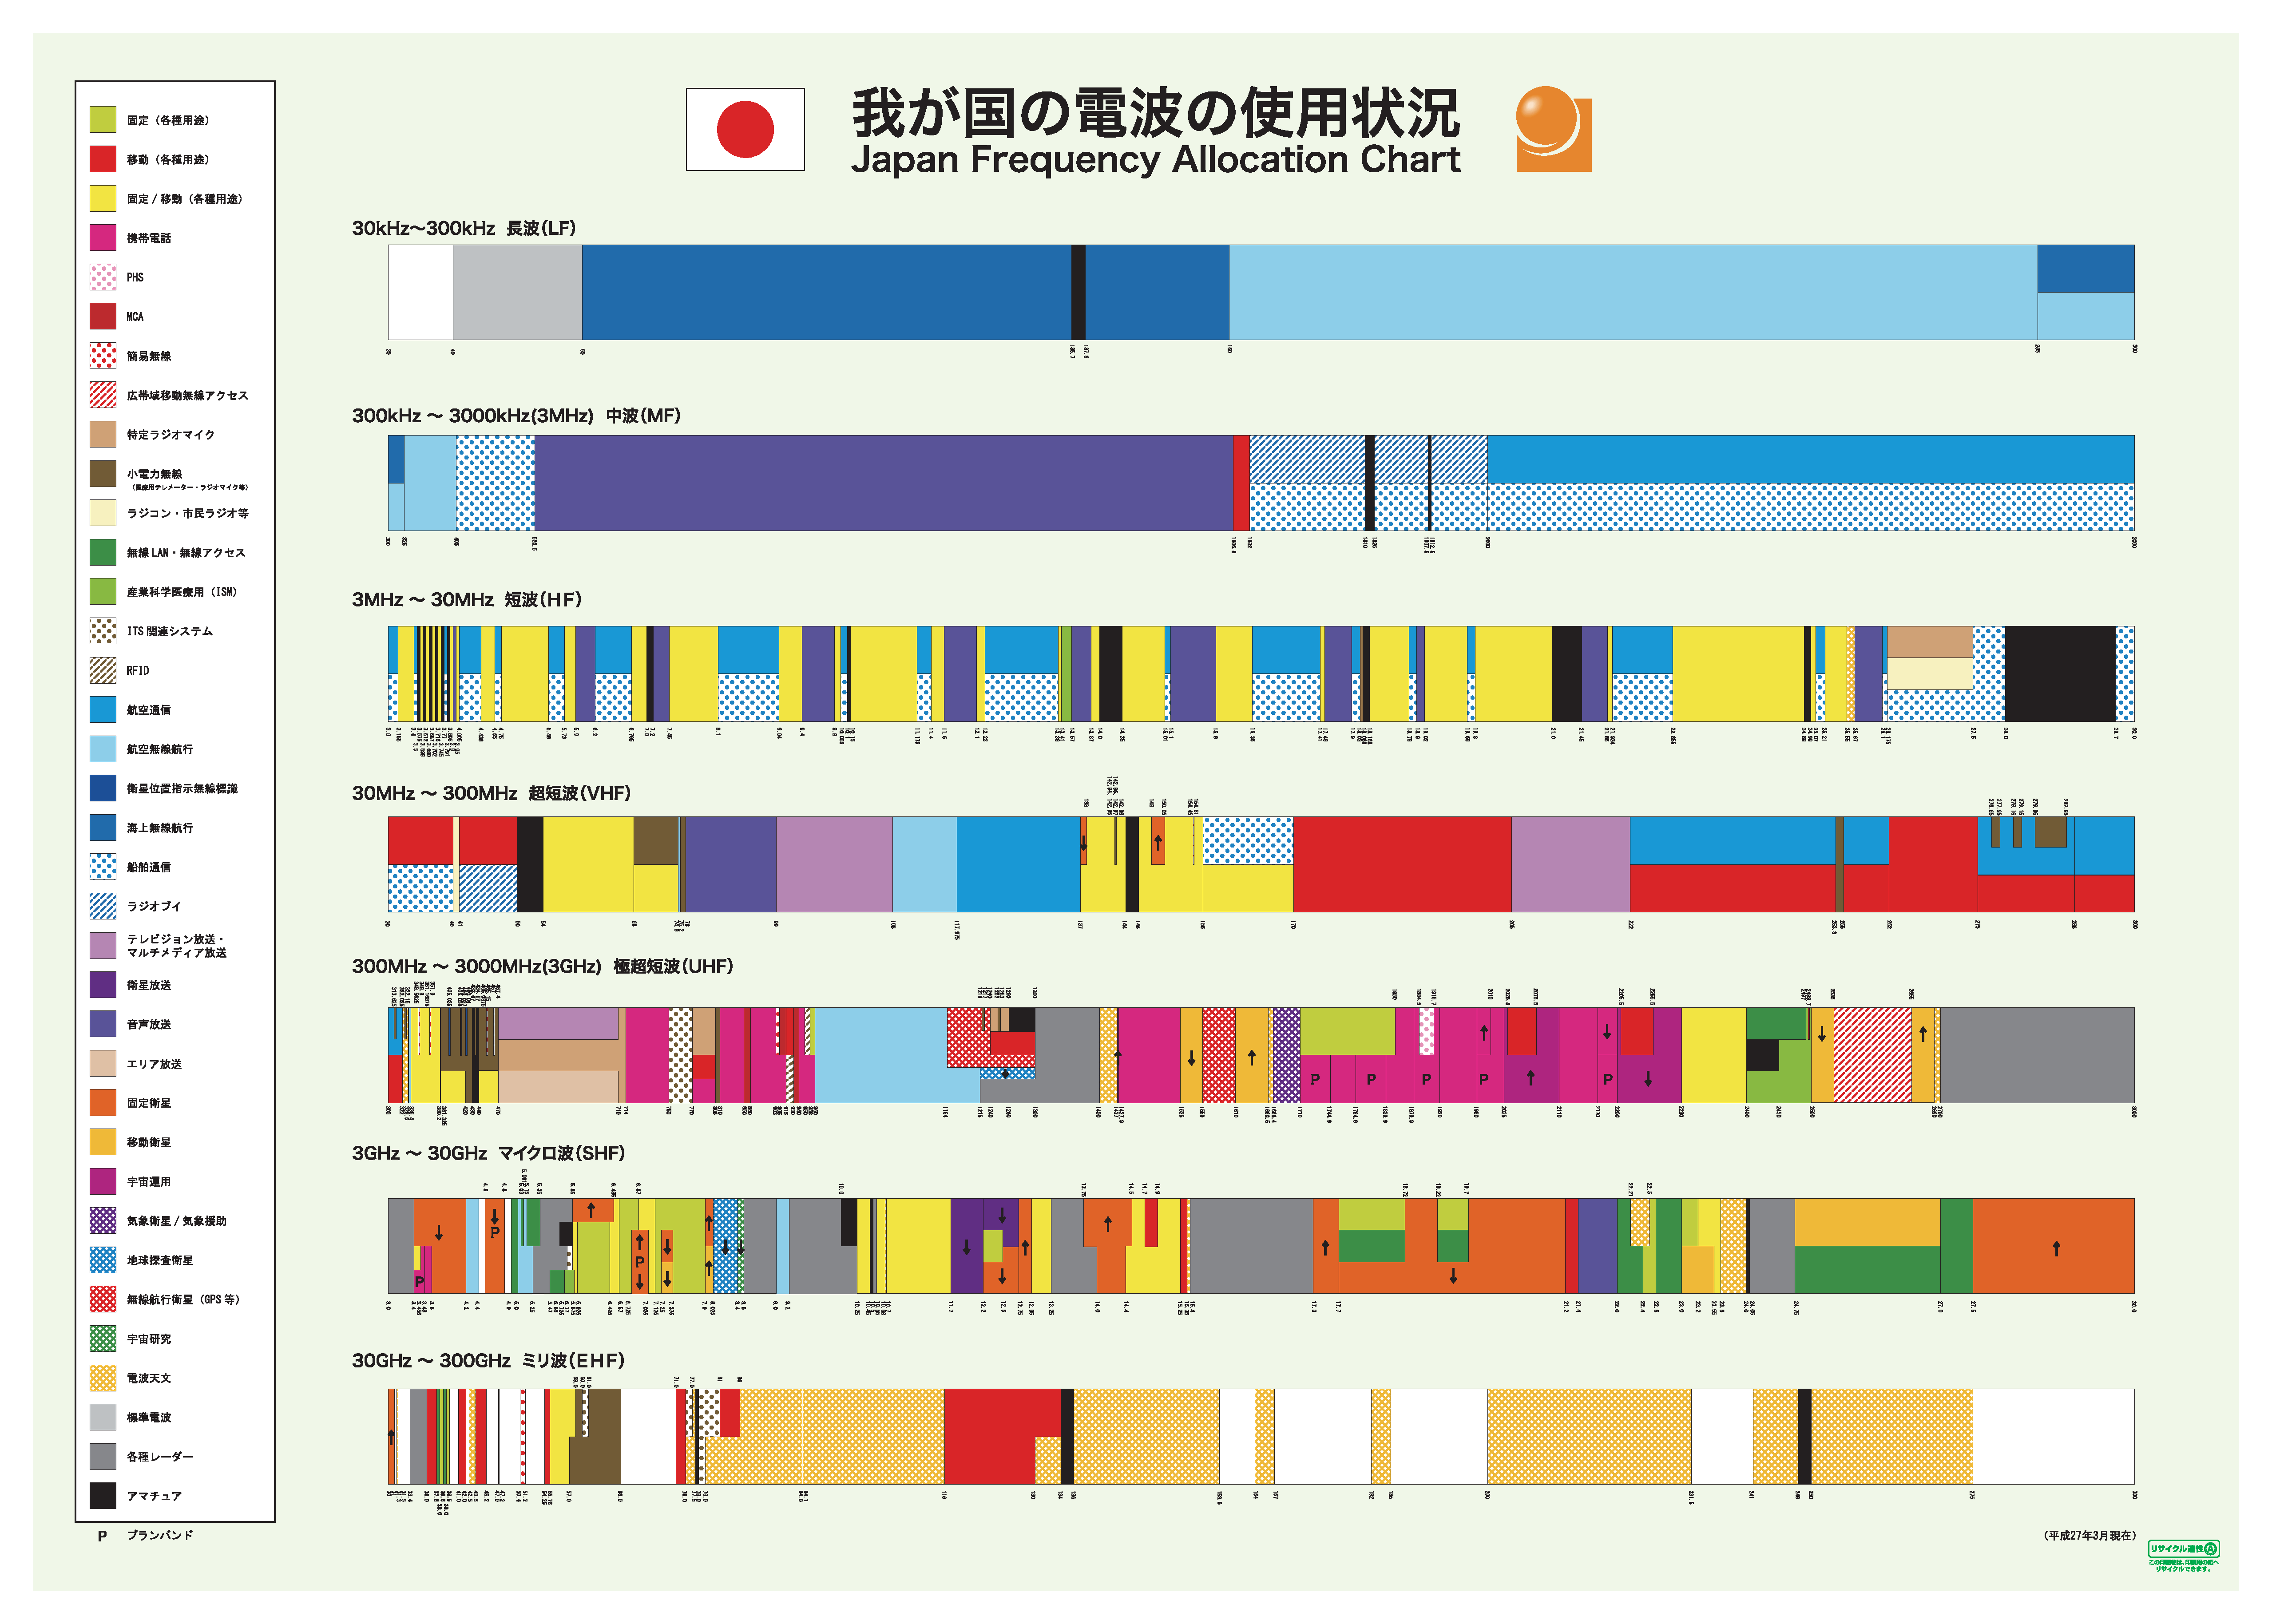
\includegraphics[width=150mm,clip]{frequency_alloc.pdf}
\caption{Japanese Frequency Allocation Chart.}
\label{fig:MIC}
\end{figure}

Since the finite spectrum resources are not able to fulfill the expoential growth of demand on traffic, it is necessary to review the present spectrum policy with fixed resource allocation for the next generation wireless communication sysytems and a effecient spectrum utilization turns to be a key problem. 

There are 2 main methods to ensure the bandwidth for new systems. Firstly, a spectrum arrangement on the whole wireless communication systems is utilized to extend available bandwidth. In 2011, an arrangement on television broadcasting is executed with switching to digital television broadcasing. However, it is not available for supporting the expoential growth of the data traffic and the number of systems. Second, an efficient utilization of bandwidth is considered  

Therefore, the idea of Dynamic Spectrum Access(DSA) is attracted attention as effective solution to the shortage of spectrum resources. 



\section{Spectrum Sharing Trend and Problem}

\section{Purpose}


